\section{Transistor come emitter follower}

Per assemblare i seguenti circuiti, non avendo più bisogno della decade di resistenze e del LED, abbiamo deciso di smontare il circuito precedente e ricominciare \emph{ex novo}.

\begin{wrapfigure}[16]{r}[0pt]{36mm}
	\caption{emitter follower semplice}
	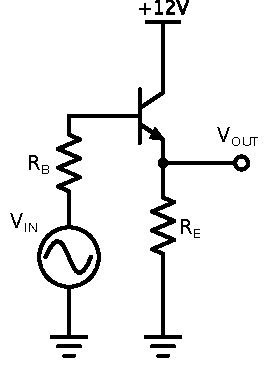
\includegraphics[height=45mm]{cc3.pdf}
	\label{fig:cc3}
\end{wrapfigure}

\subsection{emitter follower semplice}
Il nuovo circuito, mostrato in Fig. \ref{fig:cc3}, è stato alimentato tramite il generatore di forme d'onda con un'onda sinusoidale ad una tensione picco-picco $V_{pp} = \SI{10}{\volt}$.
Il valori delle reistenze usate sono $R_E = (4655.0 \pm 0.2)\,\si{\ohm}$ e $R_B = (2002.4 \pm 0.2)\,\si{\ohm}$.
Per osservare il segnale in uscita è stato collegato l'oscilloscopio all'emettitore del transistor.

Una volta collegato il circuito, abbiamo osservato che variando la frequenza tra \SI{1}{\kilo\hertz} e \SI{20}{\kilo\hertz} l'immagine mostrata a schermo dall'oscilloscopio, se escludiamo la scala temporale di riferimento, non variava.
Il segnale in output era infatti sempre in fase con il segnale in input, come si può osservare dall'immagine in Fig. \ref{fig:cc3+cc4}, che rappresenta la situazione per $f = \SI{20}{\kilo\hertz}$.
Inoltre il segnale in output (tratteggiato) è in modulo sempre minore del segnale in input.
Tale differenza è dovuta al fatto che il transistor utilizzato è formato da giunzioni p-n e, come visto nell'esperienza sul diodo, tale giunzione ha una caduta in diretta di circa $0.6\si{\volt}$. Come vediamo anche graficamente, la differenza tra segnale in input e output è di circa $0.6\si{\volt}$, per l'esattezza di $(0.607\pm0.001)\si{\volt}$.

Infine, in corrispondenza di ogni semionda negativa, in segnale in output era nullo.
Tale fenomeno è chiamato ``\emph{clipping}''. Motivazione di tale taglio è la polarizzazione della base rispetto all'emettitore. Infatti il transistor funziona finché la tensione di base è superiore di \SI{0.6}{\volt} a quella di emettitore. Avendo l'emettitore collegato a terra ($V=0$) e la base ad una $V=0+v(t)$, è immediato vedere che non appena la tensione di base è minore di \SI{0.6}{\volt} il transistor sarà interdetto e dunque la tensione rilevata dall'oscilloscopio sarà \SI{0}{\volt}.

\begin{figure}[H]
\centering
	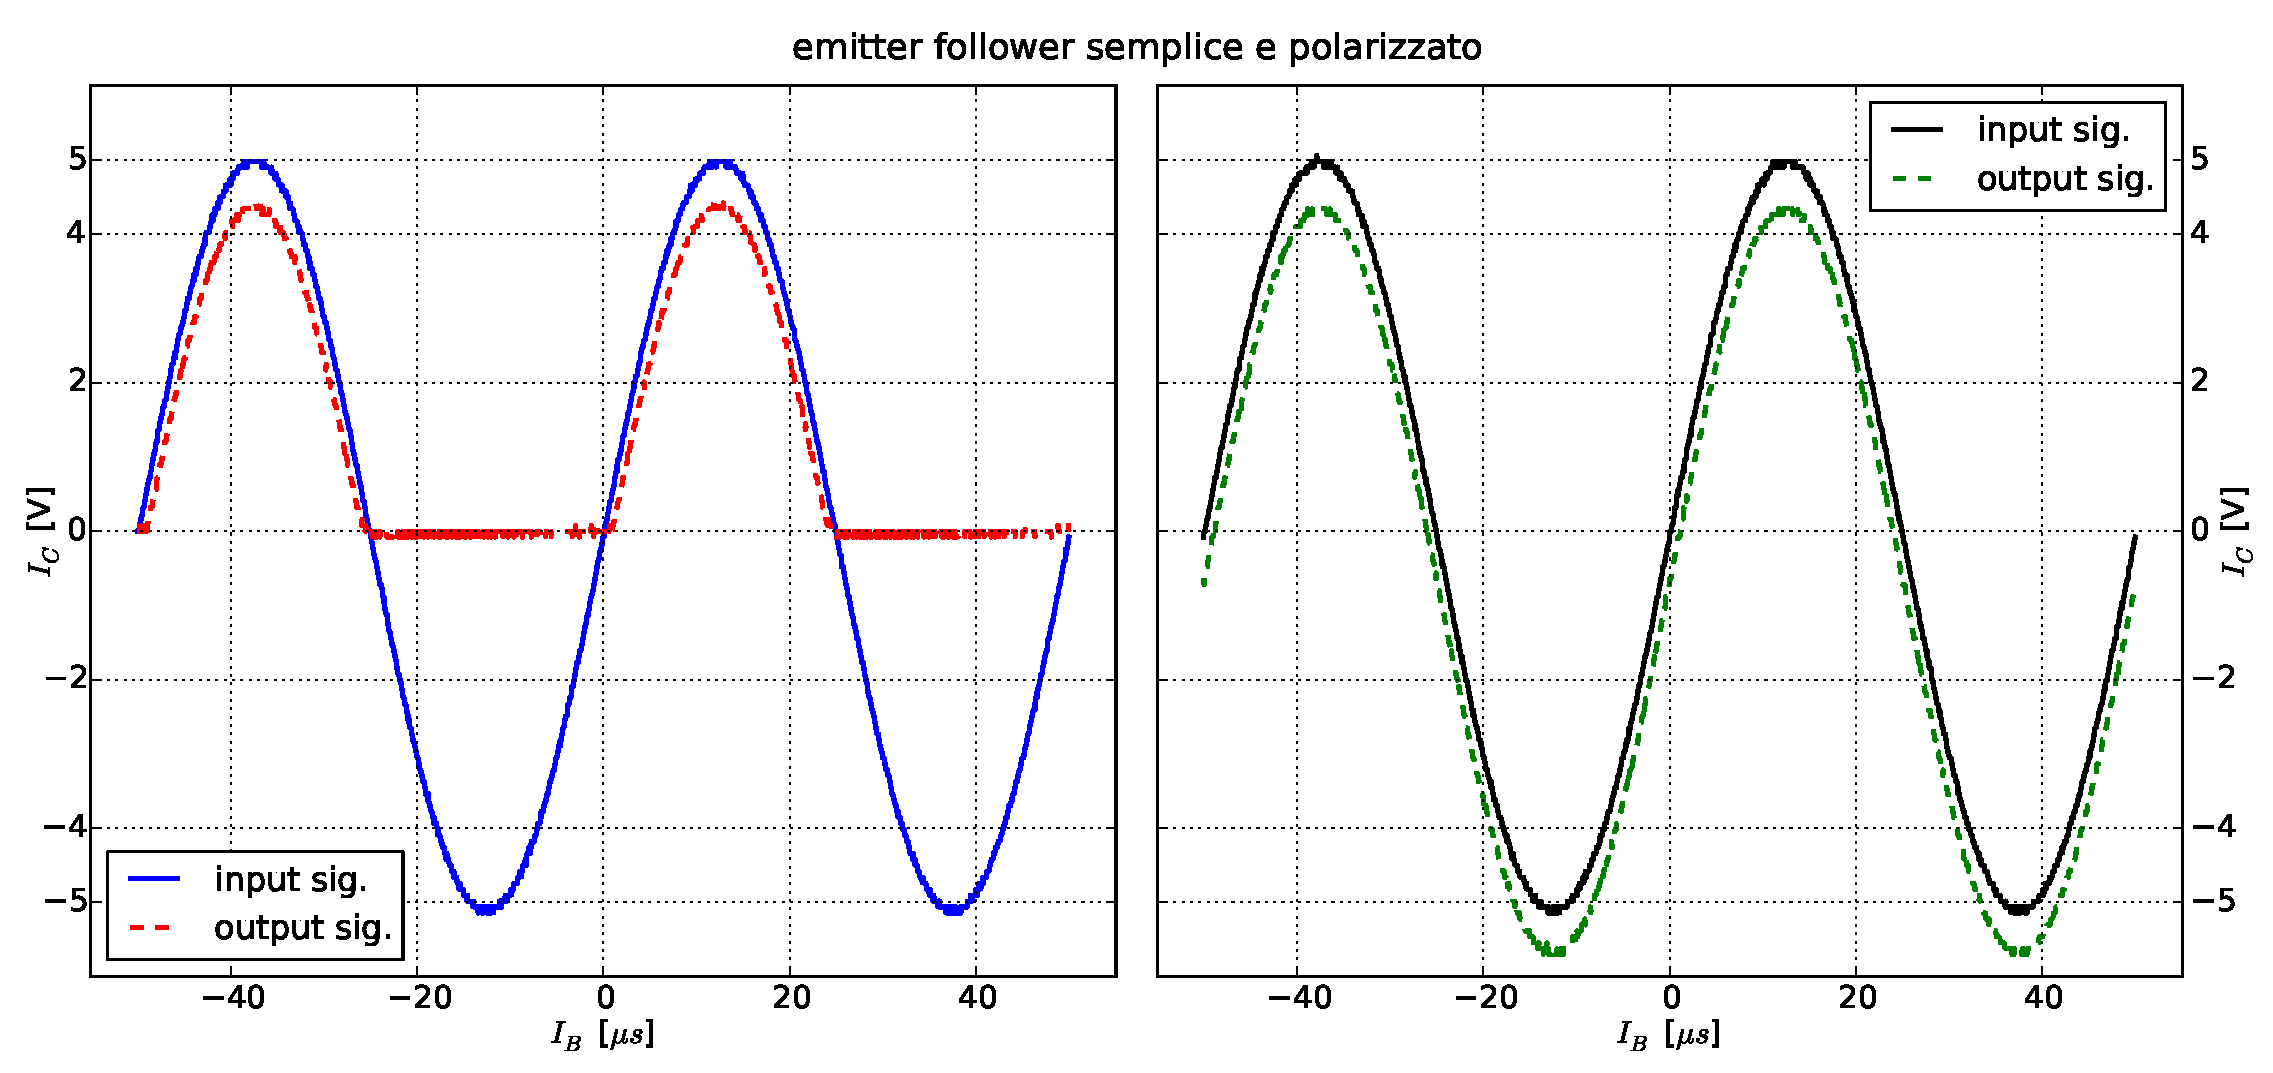
\includegraphics[width=0.81\textwidth]{cc3+cc4.pdf}
	\caption{Nel grafico a sinistra sono rappresentati i segnali in input e in output al circuito del emitter follower semplice, mentre a destra sono rappresentati i segnali dell'emitter follower polarizzato. Entrambi i segnali sono stati ricavati con una frequenza di $V_{in}$ di \SI{20}{\kilo\hertz}.}
	\label{fig:cc3+cc4}
\end{figure}

\begin{wrapfigure}[14]{l}[0pt]{36mm}
	\caption{emitter follower polarizzato}
	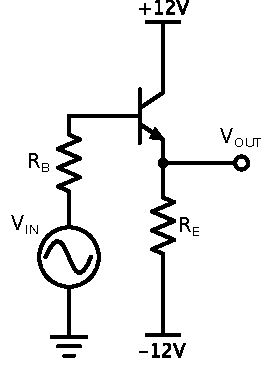
\includegraphics[height=45mm]{cc4.pdf}
	\label{fig:cc4}
\end{wrapfigure}

\subsection{emitter follower polarizzato}
Per polarizzare il transistor, come mostrato dal circuito in Fig. \ref{fig:cc4}, è bastato collegare un capo della resistenza $R_E$ al polo negativo del generatore di corrente continua anziché a terra.
I componenti circuitali sono pertanto rimasti i medesimi del circuito emitter follower ``semplice''.
Questa modifica al circuito è stata fatta per evitare, almeno parzialmente, il fenomeno di ``clipping''.

Anche in questo caso abbiamo variato la frequenza dell'onda quadra nello stesso range preso in considerazione precedentemente: il risultato è mostrato in Fig. \ref{fig:cc3+cc4}.
Ancora una volta il segnale in output è in fase con il segnale in input.
Evitando il fenomeno di ``clipping'', abbiamo ottenuto in output un segnale sinusoidale con la stessa $V_{pp}$ e stessa frequenza di quello in input, però ad una tensione minore di circa $\SI{0.6}{\volt}$. Tale fenomeno, come già detto, è dovuto alle giunzioni p-n del transistor.

\begin{wrapfigure}[17]{r}[0pt]{45mm}
	\caption{emitter follower con partitore}
	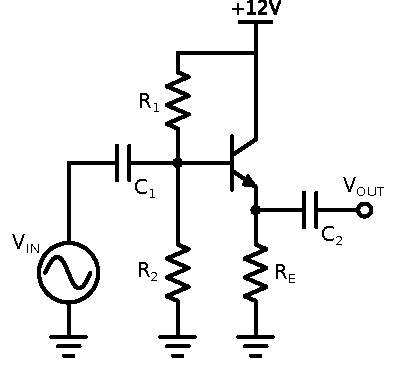
\includegraphics[height=45mm]{cc5.pdf}
	\label{fig:cc5}
\end{wrapfigure}

\subsection{emitter follower con partitore}

%\begin{figure}[H]
%\centering
%	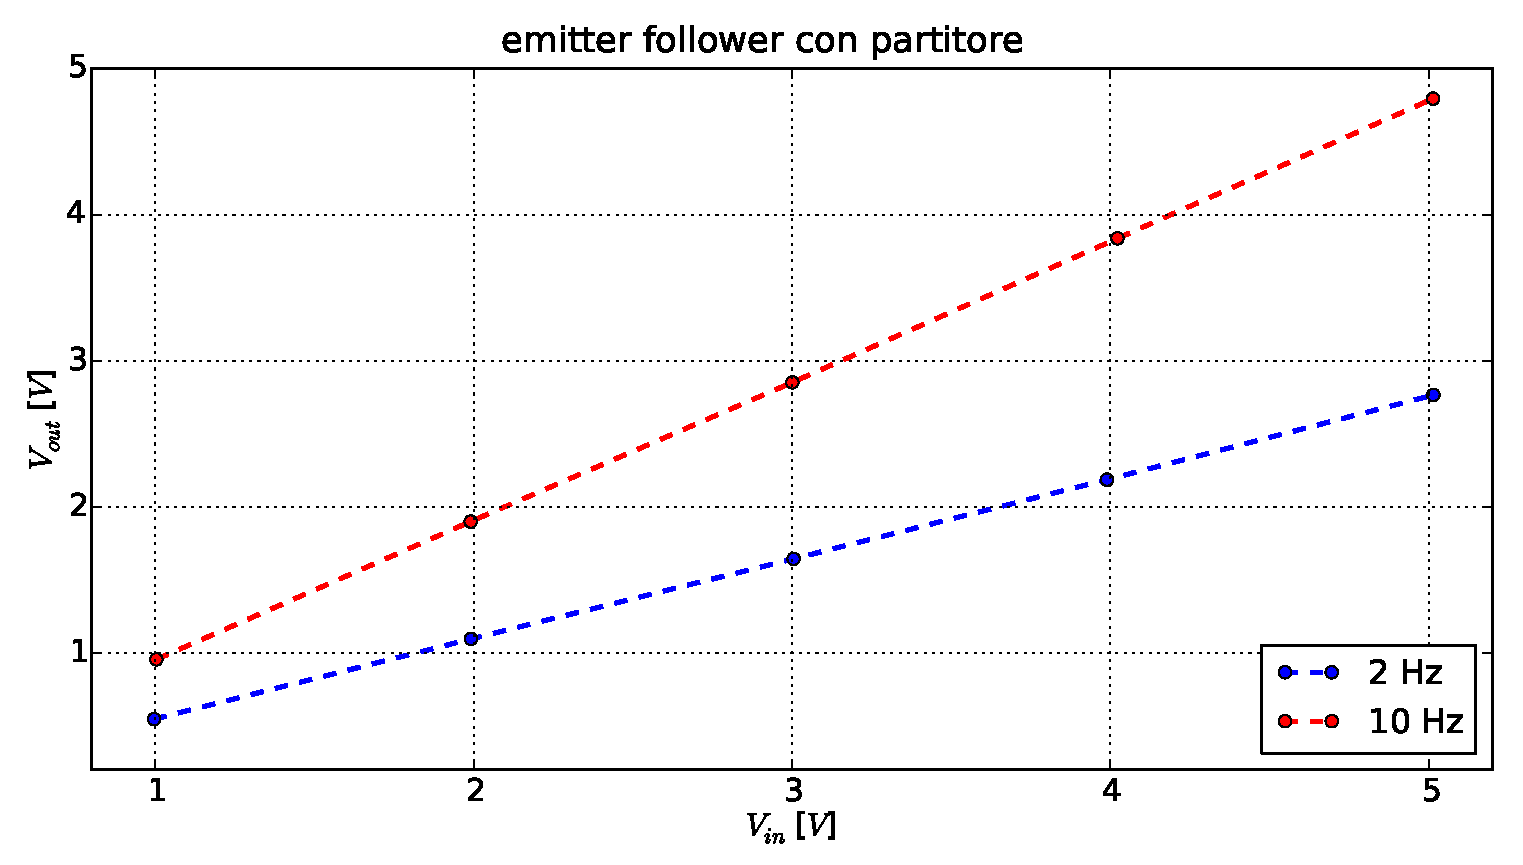
\includegraphics[width=0.7\textwidth]{am.pdf}
%	\caption{}
%	\label{fig:am}
%\end{figure}

Prima di montare il circuito riportato in Fig. \ref{fig:cc5}, abbiamo dimensionato le resistenze $R_1$ e $R_2$ del partitore in modo da avere una tensione $V_E=\frac{V_{CC}}{2}$. Dobbiamo ricordare che tra base ed emettitore abbiamo una caduta di potenziale di $0.6V$. E' dunque immediato imporre la condizione $V_B=V_E + 0.6V \rightarrow V_B=\frac{V_{CC}}{2} + 0.6V $.

Risulta immediato impostare dunque l'equazione che permette di calcolare i valori delle resistenze nel partitore:

\begin{equation}
\frac{R_2}{R_1+R_2} V_{CC}=\frac{V_{CC}}{2} + 0.6V
\label{partitore}
\end{equation}

Evidentemente i valori delle resistenze non sono univocamente determinati da Eq.(\ref{partitore}). Sarà dunque necessario utilizzare anche un'altra equazione. Una caratteristica dell'emitter follower è quella di avere un impedenza in entrata molto grande e una in uscita piccola. Tale caratteristica si realizza quando è soddisfatta la seguente equazione:

\begin{equation}
\frac{R_2}{R_1+R_2} <<\beta R_E
\label{partitore2}
\end{equation}

con $\beta$ il guadagno in corrente del transistor ed $R_E=(4.702\pm0.3)\,\si{\kilo\ohm}$. Assumendo un guadagno $\approx 100$\footnote{Non avendo ancora calcolato il guadagno del transistor dalla prima parte dell'esperienza durante la sessione di laboratorio abbiamo deciso di assumere $\beta=100$. Ai fini della bontà dell'esperimento tale scelta non è limitativa in quanto per i calcoli eseguiti conta l'ordine di grandezza.} e per molto minore $\frac{1}{10}$, otteniamo il seguente sistema:

\begin{equation}
\begin{cases}
\frac{R_2}{R_1+R_2} V_{CC}=\frac{V_{CC}}{2} + 0.6V\\
\frac{R_2}{R_1+R_2} =\frac{1}{10} 100 \cdot R_E
\end{cases}
\end{equation}

Risolvendolo algebricamente otteniamo i valori $R_1=\SI{100}{\kilo\ohm}$ e $R_2=\SI{122}{\kilo\ohm}$. I valori effettivamente utilizzati sono stati $R_1=(99.6\pm0.1)\,\si{\kilo\ohm}$ e $R_2=(122.1\pm0.2)\,\si{\kilo\ohm}$.

Avendo utilizzato un partitore, è necessario isolare il generatore di forme d'onda dal partitore stesso. Per fare ciò abbiamo dunque inserito un capacitore $C_1$ come mostrato in Fig. \ref{fig:cc5}.
\`E inoltre necessario inserire un capacitore in uscita per tagliare la componente continua di tensione dovuta alla corrente continua che scorre nell'emettitore sovrapposta al segnale variabile nel tempo. 
Avendo utilizzato un capacitore $C_1=(0.990\pm0.004)\,\si{\micro\farad}$, è necessario trovare un valore adeguato di $C_2$ in modo che la banda passante di frequenze non sia ulteriormente limitata. Per fare ciò è stata dunque trovata la frequenza di taglio dovuta al condensatore $C_1$, ricordando che essa dipende dalla costante di tempo del circuito RC:

\begin{equation}
f_t=\frac{1}{2\pi \tau} 
\label{taglio}
\end{equation}

con $\tau=C_1 \cdot (\beta R_E//R_1//R_2+R_s)$. Ricordiamo che $R_s$ è l'impedenza in uscita del generatore di forme d'onda e $\beta R_E$ l'impedenza in ingresso dell'emitter follower.

Inserendo i valori numerici otteniamo $f_t=\SI{3.3}{\hertz}$.

Invertendo Eq.(\ref{taglio}) è dunque possibile imporre la condizione di avere una frequenza di taglio uguale o minore alla $f_t$ appena trovata: 

\begin{equation}
C_2>\frac{1}{2\pi f_t R^*}
\end{equation}

Con $R^*=R_E//\frac{R_2R_1}{(R_1+R_2)(\beta +1)}$ in quanto il condensatore è sia caricato dalla resistenza $R_E$ che dall'impedenza in uscita dell'emitter follower (per comodità di calcolo è stata usata $\beta=100$). Il valore che si ottiene inserendo i dati numerici è di $C_2>\SI{320}{\micro\farad}$\footnote{Il valore di $C_2$ ottenuto con questo calcolo non è compatibile con quello utilizzato effettivamente. Infatti ci aspettavamo una frequenza di taglio di molto maggiore ai \SI{3}{\hertz} avendo utilizzato una $C_2$ circa 50 volte inferiore a quella stimata.}.

Tale valore è enorme rispetto alle capacità solitamente utilizzate. Abbiamo dunque deciso di utilizzare una capacità di $C_2=(6.728 \pm 0.005)\si{\micro\farad}$ e di controllare sperimentalmente se la frequenza di taglio era effettivamente attorno ai 150\si{\hertz}.

I dati sperimentali confermano che la capacità utilizzata non limita la frequenza di taglio del circuito. Abbiamo dunque ipotizzato che la presenza dell'oscilloscopio influenzasse la carica del condensatore. Infatti, l'oscilloscopio ha un'impedenza in ingresso $Z_{in}=1\si{\mega\ohm}$. Per stimare correttamente $C_2$ dobbiamo considerare dunque: 

$$C_2>\frac{1}{2\pi f_t R'}$$

Con $R'=Z_{in}+R^*$. In questo secondo caso otteniamo $C_2>50\,\si{\nano\farad}$.
Come vediamo, la capacità $C_2$ utilizzata non influenza assolutamente la frequenza di taglio determinata da $C_1$. 


Come già anticipato nella sezione precedente, il fenomeno di ``clipping'' avviene anche nel caso dei circuti emitter follower polarizzato ed emitter follower con partitore.
Ciò succede quando il segnale in ingresso ha un'ampiezza tale da mandare in interdizione il transistor in tutta o in parte  della semionda negativa. Ricordiamo che si può avere un effetto di ``clipping'' anche sulla semionda positiva, nel caso in cui la tensione di base superi quella di collettore. 
In Fig. \ref{fig:clip} è rappresentato il fenomeno di clipping parziale nel caso del circuito emitter follower con partitore per i valori di frequenza \SI{10}{\hertz} e tensione $V_{pp} = \SI{14}{\volt}$. Possiamo notare come la presenza dei capacitori abbia conseguenze sulla fase del segnale in uscita.


\begin{figure}[h]
\centering
	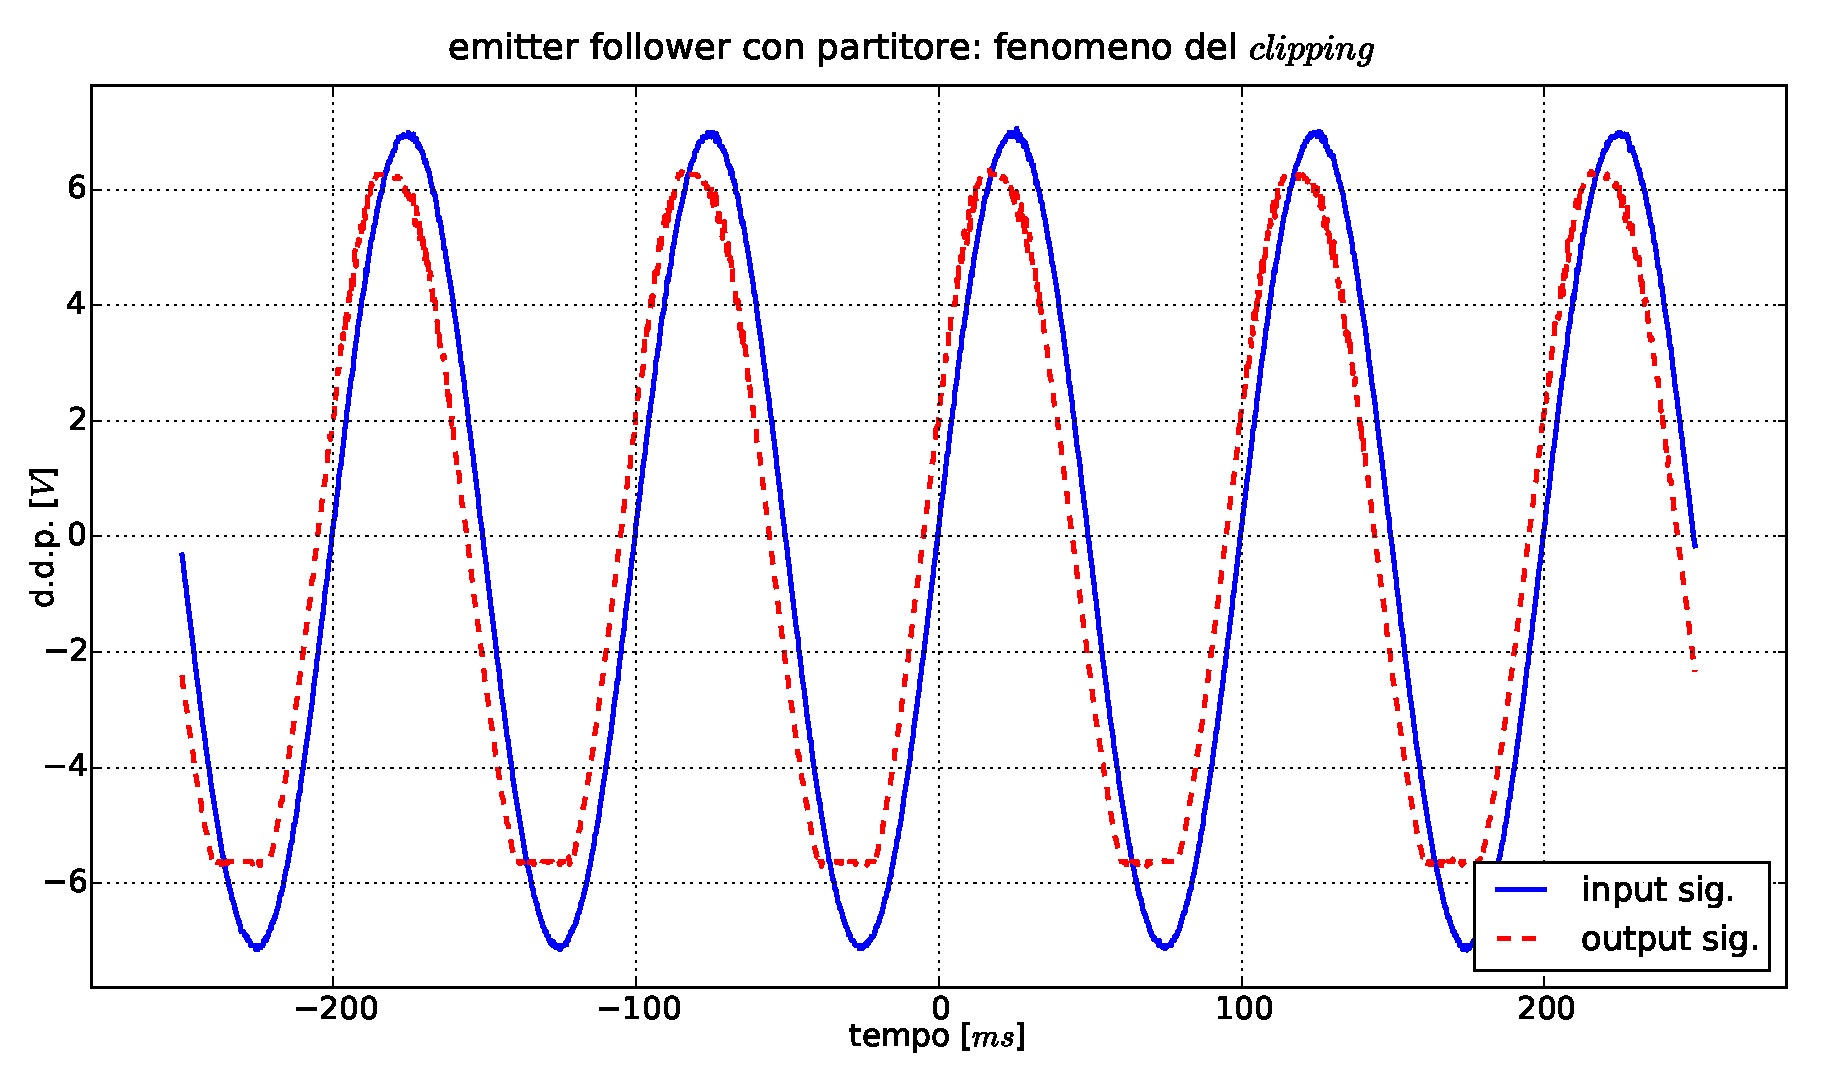
\includegraphics[width=0.7\textwidth]{clip.pdf}
	\caption{Nel grafico notiamo come il clipping riguardi solo la semiasse negativa. Ciò è dovuto al fatto che la polarizzazione della base tramite il partitore non era perfettamente simmetrica.}
	\label{fig:clip}
\end{figure}